\scanpage{45}
\[
\left\{
\begin{aligned}
f(s_i)&=0\\
\varphi(s_i,s_j)&=-(\alpha_0+2)\cdots(\alpha_{i-1}+2)
\qquad 0\leq i<j\leq n+1
\end{aligned}
\right.
\]
$f$ caractérisée par les conditions
\[
\begin{aligned}
\text{a)}\;&f\ \text{inv. par les }\tau_i\\
\text{b)}\;&f(s_0)=0\quad
(\Longleftrightarrow f\ \text{nulle sur les sommets \unsure{géom.} de }\Pi\\
\text{c)}\;&f(a_0)=1\quad
(\Longleftrightarrow \deleted{\unsure{\text{les}}}\ \text{vecteurs arêtes sont unitaires})
\end{aligned}
\]
\[
f(a_i)=(\alpha_0+2)\cdots(\alpha_{i-1}+2)\qquad0\leq i\leq n
\]
\[
\varphi(a_i,a_j)=0\qquad0\leq i<j\leq n,\quad i,j\ \text{non conséc.}
\]
\[
\varphi(a_i,a_{i+1})=-(\alpha_0+2)\cdots(\alpha_i+2)
\]
\[
\varphi(s_0,a_i)=0\qquad1\leq i\leq n
\]
\[
\varphi(s_0,a_0)=-1
\]
\[
\varphi(s_j,a_i)=0\qquad0\leq j<i\leq n,\quad
\deleted{\unsure{i<j+1}}
\]
\[
\varphi(s_j,a_{j\deleted{\unsure{+1}}})
=-(\alpha_0+2)\cdots(\alpha_{j-1}+2)
\qquad0\leq j\leq n
\]
\[
\varphi(s_j,a_{j-1})=+(\alpha_0+2)\cdots(\alpha_{j-2}+2)
\qquad1\leq j\leq n+1
\]
\deleted{$\alpha_i+2$ \unsure{inversibles}
$(0\leq i\leq n-1)\Longleftrightarrow\tau_i$}
\[
\varphi(s_j,a_i)=0\qquad0\leq i<j-1\leq n
\]
\margin{
\[
\left\{
\begin{aligned}
\varphi(s_0,s_1)&=\varphi(s_0,a_1)
\inserted{\unsure{=}\varphi(s_0,a_0)=}-1\\
\varphi(s_1,a_0)&=f(a_0)=1\\
\tau_0&\ \text{str. orth.}
\end{aligned}
\right.
\]
}
\figure{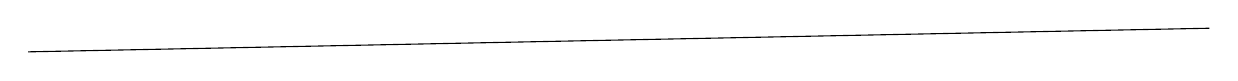
\begin{tikzpicture}\draw (0,0)--(15,0.3);\end{tikzpicture}}
$\tau_i$ réflexion strictement orthogonale
$\Longleftrightarrow(\alpha_0+2),\cdots,(\alpha_{i-1}+2)\in k^*$.
\[
(\tau_i\ \text{str. orth.}\quad\forall_{0\leq i\leq n})
\Longleftrightarrow(\alpha_i+2)\in k^*\quad\forall_{0\leq i\leq n-1}
\]
\mspage{44}

